% !TeX root = Chapter_06_Risk_Portfolio.tex
% Chapter 6 — Examining the Firm's Risk Portfolio
\documentclass[11pt,openany]{book}
\usepackage{graphicx}
\usepackage{amsmath,amssymb}
\usepackage{hanging}
\makeatletter
\def\input@path{{second_ed/style/}{../style/}}
\makeatother
\usepackage{erm_textbook_style}
\graphicspath{{second_ed/rscripts/chapter6/}{../rscripts/chapter6/}}
\providecommand{\tightlist}{\setlength{\itemsep}{0pt}\setlength{\parskip}{0pt}}
\emergencystretch=2em

\begin{document}

\setcounter{chapter}{5}
\chapter{Examining the Firm's Risk Portfolio}
\label{chap:risk-portfolio}

% -----------------------------------------------------------------------
\begin{learningobjectives}
  \item Define a firm's risk portfolio and explain why examining risks
        individually misses critical enterprise-level insights about total
        risk exposure.
  \item Construct a comprehensive risk inventory or risk register that
        systematically categorizes all material enterprise risks by type,
        exposure, and ownership.
  \item Explain correlation, covariance, and statistical dependence between
        risks, and describe how risk interdependencies affect total portfolio
        risk.
  \item Apply quantitative risk aggregation techniques, including
        variance-based aggregation and correlation-based methods, to estimate
        total enterprise risk.
  \item Understand conceptually how Monte Carlo simulation constructs
        aggregate loss distributions for the entire risk portfolio.
  \item Calculate and interpret portfolio diversification benefits, explaining
        why total portfolio risk is typically less than the sum of individual
        risks.
  \item Interpret enterprise-level Value at Risk (VaR), economic capital
        requirements, and stress test results in the context of risk appetite
        established by the board.
  \item Recognize organizational and technical challenges in implementing
        portfolio-level risk management, including data quality issues,
        correlation estimation difficulties, and siloed organizational
        structures.
\end{learningobjectives}

% -----------------------------------------------------------------------
\chapteroverview{%
In Chapters~3 and~4, we learned to identify and quantify individual risks. In
Chapter~5, we explored risk appetite---how much risk the organization is
willing to accept in pursuit of strategic objectives. A natural question now
arises: \emph{what is our total risk position across all risks?} If we know
each individual risk's magnitude, and we know our overall risk appetite, how
do we assess whether our combined exposure fits within appetite?

Answering that question requires moving from analyzing risks one at a time to
examining the firm's \emph{risk portfolio}---the totality of all material
risks the organization faces, considered together as an integrated whole. Just
as investors evaluate stocks not in isolation but as portfolios, firms must
understand how their various risks interact, combine, and potentially offset
one another.

The portfolio perspective changes risk management in three ways. First, it
reveals that total firm risk is not the sum of individual risks. When risks
are imperfectly correlated, the firm benefits from
\emph{diversification}---total portfolio risk is less than the sum of the
parts. When risks are highly correlated, the opposite happens: concentrations
and hidden dependencies create \emph{amplification effects} in which multiple
risks materialize simultaneously. The Maersk case that opens this chapter is a
vivid example of the second possibility. A single piece of malware, entering
through a tax-software update in one country, simultaneously triggered
operational, supply chain, customer service, and reputational losses across an
entire global enterprise---because all of those exposures shared a dependency
that no individual risk assessment had surfaced.

Second, portfolio analysis enables rational \emph{capital allocation}. If we
know each business unit's contribution to total portfolio risk, accounting for
correlations, we can allocate capital proportionally and require risk-adjusted
returns. Third, portfolio thinking supports better \emph{strategic decisions}.
When evaluating a new market, an acquisition, or a product launch, the
relevant question is not only ``what risk does this create?'' but ``how does
this new risk correlate with the risks we already carry?''

This chapter develops portfolio thinking systematically: defining the risk
portfolio, building the risk register, estimating correlations, aggregating
risks quantitatively, measuring diversification benefits, stress testing the
total portfolio, and connecting everything back to the risk appetite framework
of Chapter~5. A comprehensive case study walks through portfolio construction
from start to finish, and the chapter closes with the organizational and
technical challenges of making all this work in practice.%
}

\clearpage

% -----------------------------------------------------------------------
% Opening Corporate Example: Maersk and NotPetya
% -----------------------------------------------------------------------
\begin{corporateexample}[Maersk and NotPetya --- When Cyber Risk Repriced the Whole Portfolio]

In late June 2017, A.P. M\o ller--Maersk\index{Maersk}, the world's largest container
shipping company, was running 76 port terminals and about 800 vessels
worldwide, moving nearly one-fifth of global container capacity. With more
than 75{,}000 employees in 130 countries, Maersk was deeply embedded in world
trade. Cyber threats appeared on its risk maps---but as an IT problem, not as
an enterprise-level hazard capable of simultaneously crippling revenue streams
and operations across continents.

The NotPetya\index{NotPetya} malware entered Maersk's network through a seemingly routine
compliance action: a Ukrainian office used the tax software M.E.Doc, which
attackers had seeded with backdoors. Once inside, NotPetya used the
EternalBlue exploit and the Mimikatz credential-harvesting tool to jump across
unsegmented, outdated Windows machines worldwide. Within minutes, Maersk's
global operations were compromised.

The impact was immediate. Terminal operating systems serving 17 of Maersk's
76 ports were wiped clean. Shipping ground to a halt---crane operators lost
track of which containers to move, refrigerated cargo had to be managed by
hand to avoid spoilage, and normal computer-assisted coordination vanished. At
the Port of Los Angeles, Maersk's APM Terminal closed for days while ships
queued at anchor. Booking systems went down. The company resorted to paper
records and consumer messaging apps in an effort to keep cargo moving.

As IT teams scrambled to disconnect the network and begin recovery, they
discovered that the attack had wiped out every global domain controller.
Maersk had assumed its synchronized backups provided resilience; it had not
planned for simultaneous erasure. Global restoration became possible only when
a single offline backup was located---on a server in Ghana that had lost power
during the attack. An employee physically carried the hard drive from Ghana to
Nigeria, then to the United Kingdom, where recovery operations finally began.
Rebuilding 4{,}000 servers and 45{,}000 PCs took about ten days; lingering
effects lasted months.

The financial losses were severe. Maersk reported \$200--300~million in direct
impacts---a figure widely believed by staff to be conservative. The White
House, attributing the attack to Russia, later cited \$10~billion in total
global damages across all affected firms. The deeper lesson was structural:
NotPetya disrupted multiple Maersk businesses at once, from logistics and port
operations to internal booking systems, demonstrating how a ``technical''
cyber risk\index{cyber risk} could trigger system-wide, correlated losses across operational,
financial, and reputational lines.

After the event, Maersk overhauled its technology portfolio and its risk
approach---approving nearly every new cyber defense its staff requested,
including rapid upgrades, network segmentation, and robust, geographically
distributed backups. Leadership recast resilience not merely as risk
management but as a source of competitive advantage.

Maersk's NotPetya experience stands as a striking documentation of how digital
attacks can cause globally linked business interruptions, and as a lesson in
the need for true portfolio-wide risk assessment---especially of latent
dependencies that only a system shock reveals.

\source{Columbia University School of International and Public Affairs (2022);
Greenberg (2018a, 2018b); Los Angeles Times (2017).}

\end{corporateexample}

% -----------------------------------------------------------------------
\section{From Individual Risks to Portfolio Perspective}
\label{sec:portfolio-perspective}
% -----------------------------------------------------------------------

\subsection{The Limits of Individual Risk Analysis}
\label{subsec:limits-individual}

Traditional risk management operates in silos\index{siloed risk management}. Treasury manages foreign
exchange and interest rate risk. The insurance department manages property,
liability, and workers' compensation. IT manages cybersecurity. Each function
identifies, measures, and mitigates its risks using specialized expertise and
tools.

The specialized approach has real advantages---deep expertise, focused
attention, clear accountability. But managing risks in isolation creates
predictable blind spots.

\textbf{Failure to see aggregate exposure.} An organization might conclude
that each individual risk is acceptable in isolation yet face unacceptable
total exposure. Before June 2017, Maersk could have looked at its cyber risk,
its port operations risk, its customer service exposure, and its reputational
risk separately and judged each one manageable. What no silo could see was
that all four shared a single point of failure: an unsegmented global IT
network. The same pattern appears in less dramatic settings. A manufacturer
may find property risk, product liability risk, and supply chain risk each
manageable individually---until a single earthquake in a region containing its
facilities, suppliers, and customers triggers all three at once.

\textbf{Missed diversification opportunities.} Managing risks separately also
hides natural offsets. A global company with euro revenues and dollar costs
holds a natural currency hedge---recognizing it might reduce hedging costs. A
company with both growth and defensive businesses may find that portfolio
volatility is lower than either business alone because their earnings move
differently across the economic cycle.

\textbf{Suboptimal capital allocation.} Without understanding each risk's
contribution to total portfolio risk, organizations allocate capital
inefficiently. A business unit generating high returns while adding little to
total portfolio risk (because its risks are uncorrelated with everything else)
deserves more capital than a unit with comparable returns but highly
correlated risks that amplify total exposure.

\textbf{Inability to assess risk appetite compliance.} Risk appetite is
typically defined at the enterprise level---maximum acceptable annual loss,
minimum capital ratio, maximum earnings volatility. Determining whether the
organization actually operates within appetite requires aggregating all risks
into a total exposure. Individual risk assessments cannot answer an
enterprise-level question.

\subsection{The Portfolio Metaphor from Finance}
\label{subsec:portfolio-metaphor}

The intellectual foundation for portfolio risk management comes from modern
portfolio theory\index{modern portfolio theory}. Harry Markowitz\index{Markowitz, Harry} demonstrated in 1952 that investors should
evaluate securities not by their individual risk-return characteristics but by
their contribution to portfolio risk and return. The key insight:
\textbf{diversification reduces risk} when asset returns are imperfectly
correlated.

A simple example makes the point. An investor holds two stocks, each with
expected return of 10\% and standard deviation of 20\%. If the stocks are
perfectly correlated, the portfolio also has a 20\% standard deviation. If
they are uncorrelated, portfolio standard deviation falls to 14.1\%---a 29\%
reduction in risk with no sacrifice in expected return. The benefit arises
purely from combining imperfectly correlated assets.

Enterprise risk management applies the same logic to corporate risks. A
retailer facing both demand uncertainty and commodity cost uncertainty might
find that recessions reduce demand and commodity prices together, so falling
costs partially offset falling sales. That negative correlation is a natural
hedge\index{natural hedge}---invisible to anyone studying either risk alone.

The portfolio perspective transforms risk management from defensive
loss-prevention into strategic risk optimization: selecting the combination of
risks that best supports objectives given constraints on capacity and
appetite.

\subsection{What Changes with Portfolio Thinking}
\label{subsec:portfolio-shifts}

Adopting a portfolio perspective requires several conceptual shifts.

\textbf{From minimizing individual risks to optimizing total risk.} Risk
management is not about eliminating every exposure. Some risks create value
and should be pursued; others are byproducts of the business model and should
be managed efficiently. Portfolio thinking asks: given our strategy, what
combination of risks optimizes risk-adjusted value creation within our
capacity and appetite?

\textbf{From risk mitigation to risk allocation.} Instead of viewing risk
management primarily as buying insurance or hedging exposures, portfolio
thinking emphasizes how much risk to allocate to each activity. Capital
allocation becomes a risk management tool---units that deliver superior
risk-adjusted returns and contribute favorably to diversification receive more
capital.

\textbf{From point-in-time assessment to dynamic monitoring.} A risk portfolio
is not static. Business mix changes, market conditions evolve, new risks
emerge. Portfolio risk management requires continuous monitoring of exposures,
correlations, and concentrations, with periodic rebalancing.

\textbf{From functional silos to enterprise integration.} Treasury, insurance,
IT, operations, and business units must share data, coordinate analysis, and
accept enterprise-level decisions even when those decisions disadvantage
individual units. This is usually the hardest shift of the four, and we return
to it in Section~\ref{sec:implementation}.

% -----------------------------------------------------------------------
\section{What Is a Risk Portfolio?}
\label{sec:what-is-portfolio}
% -----------------------------------------------------------------------

\subsection{Defining the Risk Portfolio}
\label{subsec:defining-portfolio}

A firm's \textbf{risk portfolio}\index{risk portfolio} is the totality of all material risks the
organization faces, considered together as an integrated system. The portfolio
includes:

\textbf{All material risk types:} financial risks (market, credit, liquidity),
operational risks (process failures, technology, human error), hazard risks
(property damage, liability, business interruption), strategic risks
(competitive threats, innovation failures, M\&A), and compliance and
regulatory risks.

\textbf{Quantified exposures:} for each risk, measures of exposure---expected
loss, standard deviation, Value at Risk, or other metrics from the assessment
process (Chapter~4).

\textbf{Risk interdependencies:} correlations, dependencies, and potential
interactions between risks. This is what distinguishes portfolio analysis from
merely listing risks.

\textbf{Risk ownership and accountability:} each material risk should have an
identified owner\index{risk owner}---a business unit, function, or individual responsible for
managing that risk within established limits.

\subsection{Risk Categories in the Portfolio}
\label{subsec:risk-categories}

Most organizations organize their portfolios using taxonomies that group
similar risks. Common frameworks include:

\textbf{COSO ERM categories}\index{COSO} (COSO, 2017):
\begin{itemize}\tightlist
  \item Strategic risks (affecting strategy and objectives)
  \item Operations risks (affecting operational execution)
  \item Reporting risks (affecting reliability of information)
  \item Compliance risks (affecting adherence to laws and regulations)
\end{itemize}

\textbf{Financial services industry categories:}
\begin{itemize}\tightlist
  \item Credit risk
  \item Market risk (interest rate, foreign exchange, equity, commodity)
  \item Liquidity risk
  \item Operational risk
  \item Insurance/underwriting risk (for insurers)
  \item Strategic/business risk
\end{itemize}

\textbf{Categorization by controllability:}
\begin{itemize}\tightlist
  \item Controllable risks (process risks, quality risks, human error)
  \item Partially controllable risks (customer credit risk, vendor reliability)
  \item External risks (market prices, natural disasters, regulatory changes)
\end{itemize}

The specific taxonomy matters less than \textbf{comprehensive coverage} (no
material risks overlooked) and \textbf{consistency} (everyone uses the same
definitions and classifications).

\subsection{Materiality: What Belongs in the Portfolio?}
\label{subsec:materiality}

Not every conceivable risk belongs in the portfolio---only \textbf{material}
risks that could significantly affect objectives or threaten viability.
Materiality criteria typically include \emph{financial magnitude} (risks that
could generate losses exceeding a threshold---1\% of revenue, 5\% of capital,
or specific dollar amounts), \emph{strategic importance} (risks that, even if
financially modest, could affect competitive position, reputation, or
strategic objectives), \emph{regulatory significance} (risks regulators
explicitly require the organization to assess and manage), and
\emph{stakeholder concern} (risks important to investors, rating agencies,
customers, or other stakeholders, even if management views them as minor).

A practical approach establishes materiality thresholds\index{materiality threshold} during risk
identification (Chapter~3) and includes in the portfolio all risks meeting any
criterion. For large organizations, the portfolio might contain 20--50
material risks; for smaller or simpler firms, 10--15 might suffice.

% -----------------------------------------------------------------------
\section{Why Risk Aggregation Matters for Enterprise Decision-Making}
\label{sec:why-aggregation}
% -----------------------------------------------------------------------

Risk aggregation\index{risk aggregation}---combining individual risks into a total portfolio
view---serves three enterprise purposes.

\subsection{Economic Capital and Capital Allocation}
\label{subsec:economic-capital-allocation}

\textbf{Economic capital}\index{economic capital} is the amount of capital the firm needs to hold to
remain solvent at a specified confidence level given its total risk profile.
Unlike regulatory capital (which follows standardized formulas), economic
capital reflects the firm's actual risks and their interactions.

Calculating economic capital requires aggregation:

\begin{enumerate}\tightlist
  \item Measure each individual risk (expected loss and distribution shape)
  \item Estimate correlations between risks
  \item Aggregate risks to determine the total loss distribution
  \item Economic capital = loss threshold at the chosen confidence level
        (e.g., 99.5\% VaR) minus expected loss
\end{enumerate}

Example: a bank assesses three major risk types:
\begin{itemize}\tightlist
  \item Credit risk: expected loss \$50M, VaR(99\%) = \$200M
  \item Market risk: expected loss \$10M, VaR(99\%) = \$80M
  \item Operational risk: expected loss \$15M, VaR(99\%) = \$100M
\end{itemize}

If the bank simply summed VaRs, it would need \$380M of capital. But if these
risks are imperfectly correlated (credit--market correlation 0.4,
credit--operational 0.2, market--operational 0.1), aggregation yields
portfolio VaR(99\%) of about \$280M---roughly \$100M less than the simple sum.
That \$100M is the \textbf{diversification benefit}\index{diversification benefit}: the savings from risks
not materializing simultaneously.

Once economic capital is determined at the portfolio level, it can be
\textbf{allocated} to business units based on each unit's contribution to
total portfolio risk. Units that add substantial risk relative to their
earnings should receive less capital or be required to generate higher returns
on what they receive.

\subsection{Risk Appetite Compliance}
\label{subsec:appetite-compliance}

Risk appetite\index{risk appetite!compliance} (Chapter~5) is typically stated in enterprise-level terms:
``annual losses shall not exceed 15\% of capital with 95\% confidence''; ``we
will maintain a Tier~1 capital ratio of at least 10\%.'' Assessing compliance
requires knowing \textbf{total portfolio risk}, not just individual risks. A
firm might be within appetite on every individual risk yet exceed appetite in
aggregate.

This is exactly the machinery the adidas\index{adidas} case in Chapter~5 described: the
company aggregated its risk portfolio using stochastic simulation and compared
total exposure against both its risk appetite (95\% threshold) and its risk
capacity (99\% threshold). Aggregation is what converts an appetite statement
from aspiration into a testable constraint.

Example: a manufacturer sets appetite at ``maximum annual loss of \$100M with
95\% confidence'' and faces four major risks with individual VaR(95\%) of
\$40M, \$35M, \$30M, and \$25M. The simple sum is \$130M---apparently over
appetite. But if the risks are largely uncorrelated (a product defect tells
you nothing about a cyber attack), proper aggregation might yield portfolio
VaR(95\%) = \$75M, comfortably within appetite. Without aggregation,
management might unnecessarily reduce risks that are perfectly acceptable in
portfolio context.

The reverse error is worse. If the same four risks were concentrated in a
single earthquake-prone region, portfolio VaR could approach the full \$130M.
Failure to aggregate would create false comfort---each risk ``within
appetite'' individually while the enterprise sat well outside it. Maersk's
experience was a version of this error: each affected business line's exposure
looked tolerable on its own; the shared IT dependency made the true aggregate
exposure enormous.

\subsection{Strategic Decisions and Portfolio Optimization}
\label{subsec:strategic-decisions}

Major strategic decisions change the risk portfolio:

\begin{itemize}\tightlist
  \item \textbf{Acquisitions} add the target's risks; correlations determine
        whether the deal increases or decreases total risk
  \item \textbf{New market entry} adds market-specific risks; geographic
        diversification may reduce total risk if the new market is
        uncorrelated with existing ones
  \item \textbf{Product line expansion} adds product-specific risks;
        diversification into uncorrelated products reduces total risk
  \item \textbf{Divestitures} remove risks; selling a highly correlated
        business may not reduce total risk proportionally
\end{itemize}

Example: a U.S.-based manufacturer considers two expansion strategies.
\textbf{Option~A} expands U.S. manufacturing capacity to serve growing
domestic demand. \textbf{Option~B} builds manufacturing in Asia to serve Asian
markets.

Option~A adds capacity and market risk highly correlated with the existing
U.S. business---same economy, same demand drivers. If the U.S. economy
weakens, both existing and new operations suffer together. Option~B adds risks
tied to Asian economic conditions, likely less correlated with U.S.
operations. Asian demand may hold up when U.S. demand weakens, or vice versa.

The choice depends on strategy, but portfolio analysis makes the trade-off
explicit: Option~A is simpler but concentrates risk; Option~B is more complex
but diversifies it. Management can make an informed decision only with
portfolio-level analysis.

% -----------------------------------------------------------------------
\section{Mapping and Inventorying the Firm's Risk Portfolio}
\label{sec:risk-register}
% -----------------------------------------------------------------------

Constructing a risk portfolio begins with a systematic inventory of all
material risks. The output is a \textbf{risk register}\index{risk register}---a structured database
documenting each risk.

\subsection{Building the Risk Register}
\label{subsec:building-register}

A comprehensive risk register includes, for each material risk:

\textbf{Risk identification information:} a unique identifier (R01, R02,
etc.); a short descriptive name (``Commercial credit risk,'' ``Cyber data
breach''); a category from the established taxonomy; and a brief narrative
describing the risk and its potential consequences.

\textbf{Risk ownership and accountability:} the risk owner (business unit,
function, or individual accountable for managing the risk) and the
second-line risk management or compliance function providing oversight.

\textbf{Risk exposure metrics:} expected annual loss; standard deviation;
Value at Risk (95\% or 99\%); maximum possible loss; and current exposure
(loan portfolio size, insured values, transaction volumes).

\textbf{Qualitative assessments:} likelihood rating (Low, Medium, High,
Critical); impact rating (Minor, Moderate, Major, Catastrophic); risk velocity
(how quickly the risk can materialize); and controllability.

\textbf{Risk response and control information:} key controls or mitigants in
place; residual risk after controls; and the treatment strategy (avoid,
reduce, transfer, accept).

\textbf{Risk correlation notes:} qualitative or quantitative assessment of
dependencies with other risks, and common external drivers affecting multiple
risks.

\subsection{Risk Register Example}
\label{subsec:register-example}

Table~\ref{tab:risk-register} illustrates a partial risk register for a
mid-sized manufacturing company.

\begin{ermtable}{Partial risk register for a mid-sized manufacturing company}[tab:risk-register]
\begin{tabularx}{\textwidth}{@{}clllrrY@{}}
\toprule
\textbf{ID} & \textbf{Risk Name} & \textbf{Category} & \textbf{Owner} &
\textbf{Exp.\ Loss} & \textbf{VaR(95\%)} & \textbf{Key Correlations} \\
\midrule
R01 & Product liability & Operational & COO & \$8M & \$40M & High corr.\ w/ R04 \\
R02 & Property damage & Hazard & Facilities & \$5M & \$35M & High corr.\ w/ R03 \\
R03 & Business interruption & Hazard & Facilities & \$12M & \$45M & High corr.\ w/ R02 (0.9) \\
R04 & Product recalls & Operational & Quality & \$6M & \$50M & High corr.\ w/ R01 \\
R05 & Cyber data breach & Operational & IT & \$3M & \$25M & Mod.\ corr.\ w/ R06 \\
R06 & Reputational damage & Strategic & CEO & \$10M & \$60M & Many correlations \\
R07 & Supply chain disruption & Operational & Supply Chain & \$15M & \$55M & Mod.\ corr.\ w/ R02, R03 \\
R08 & Foreign exchange risk & Market & Treasury & \$4M & \$20M & Low corr.\ w/ operations \\
R09 & Interest rate risk & Market & Treasury & \$2M & \$15M & Low corr.\ w/ operations \\
R10 & Key talent loss & Strategic & HR & \$5M & \$30M & Low corr.\ w/ most risks \\
\bottomrule
\end{tabularx}
\tablenote{Likelihood and impact ratings omitted for space. Expected loss and
VaR figures are annual.}
\end{ermtable}

Several patterns are worth noticing:

\begin{itemize}\tightlist
  \item \textbf{Property damage (R02) and business interruption (R03) are
        highly correlated} because the same event---fire, natural
        disaster---typically causes both
  \item \textbf{Product liability (R01) and recalls (R04) correlate strongly}
        because defective products drive both
  \item \textbf{Financial market risks (R08, R09) correlate weakly with
        operational risks}, providing diversification
  \item \textbf{Reputational risk (R06) potentially correlates with many
        risks} because nearly any failure can damage reputation
\end{itemize}

\subsection{The Risk Mapping Process}
\label{subsec:mapping-process}

Building the register is an ongoing enterprise process, not a one-time
exercise:

\begin{enumerate}\tightlist
  \item \textbf{Annual comprehensive review:} risk committees or the ERM
        function conduct enterprise-wide risk identification using the methods
        of Chapter~3---workshops, scenario analysis, SWOT, review of 10-K risk
        factors.
  \item \textbf{Quarterly updates:} business unit leaders and risk owners
        update exposures, reassess likelihood and impact, and note changes in
        correlations or controls.
  \item \textbf{Event-triggered updates:} acquisitions, divestitures, new
        product launches, significant losses, and regulatory changes trigger
        immediate updates.
  \item \textbf{Validation and challenge:} second-line functions (ERM,
        internal audit) validate that the register is complete, the metrics
        reasonable, and the correlations properly assessed.
  \item \textbf{Board oversight:}\index{board of directors!risk oversight} the board risk committee reviews the
        register at least annually, confirming that all material risks are
        identified and aggregate exposure aligns with appetite.
\end{enumerate}

\subsection{Common Pitfalls in Risk Inventories}
\label{subsec:register-pitfalls}

Several problems routinely undermine risk registers.

\textbf{Incomplete coverage.} Emerging risks get missed because they don't fit
traditional categories---cyber risk before it was widely recognized, climate
risk, pandemic risk. Maersk's pre-2017 risk maps included cyber threats; what
they missed was the enterprise-wide dependency structure that turned an IT
incident into a global business interruption.

\textbf{Inconsistent measurement.} If credit risk is measured as VaR(95\%) and
operational risk as maximum loss, they cannot be compared or aggregated.

\textbf{Stale information.} Registers created once and never updated lose
relevance rapidly.

\textbf{Lack of granularity.} Defining risks too broadly (``operational
risk'') without breaking them into components loses useful information.

\textbf{Ignoring correlations.} Treating related risks as independent leads to
underestimating total portfolio risk---the most consequential error of the
five.

A well-maintained register is the foundation for everything that follows:
aggregation, stress testing, capital allocation, and appetite compliance
monitoring.

% -----------------------------------------------------------------------
\section{Understanding Risk Correlations and Dependencies}
\label{sec:correlations}
% -----------------------------------------------------------------------

Correlation is the statistical concept that distinguishes portfolio analysis
from risk listing. Understanding how risks move together---or fail
to---is essential for estimating total portfolio risk.

\subsection{Correlation: Definition and Interpretation}
\label{subsec:correlation-definition}

\textbf{Correlation}\index{correlation} (denoted \(\rho\), the Greek letter rho) measures the
degree to which two variables move together, ranging from \(-1\) to \(+1\):

\textbf{\(\rho = +1\) (perfect positive correlation):} the two risks always
move together and proportionally. Perfectly correlated risks provide zero
diversification benefit---they are effectively the same risk. Example:
property damage and business interruption from the same hurricane are nearly
perfectly correlated; in practice \(\rho \approx 0.9\) to \(1.0\).

\textbf{\(\rho = 0\) (zero correlation):} the risks move independently.
Knowing one outcome tells you nothing about the other. Zero-correlated risks
provide maximum diversification benefit. Example: whether a company
experiences a data breach tells you nothing about whether oil prices will
rise.

\textbf{\(\rho = -1\) (perfect negative correlation):} the risks always move
in opposite directions. Negative correlation creates natural hedges. Example:
a company with euro revenues and dollar costs---euro appreciation increases
revenue value while dollar costs hold steady. In practice \(\rho\) is rarely
close to \(-1\).

\textbf{Intermediate positive correlation (\(0 < \rho < 1\)):} most business
risk pairs fall here. Example: credit risk and market risk at a bank often
correlate around 0.3 to 0.5---economic downturns hurt both markets and
borrowers, but some defaults occur for idiosyncratic reasons.

\subsection{Why Correlation Affects Portfolio Risk}
\label{subsec:correlation-portfolio-risk}

Correlation determines whether total portfolio risk is greater than, equal to,
or less than the sum of its parts. For a portfolio with two risks:

\[
\text{Portfolio Variance} = \sigma_1^2 + \sigma_2^2 + 2\rho\,\sigma_1\sigma_2
\]

The third term---the \textbf{covariance term}\index{covariance}---does the work:

\begin{itemize}\tightlist
  \item If \(\rho = 0\), the covariance term vanishes and portfolio variance
        is just the sum of individual variances. Diversification appears
        because standard deviation grows with the square root of variance, not
        linearly.
  \item If \(\rho = +1\), the covariance term is maximized and portfolio
        standard deviation equals the sum of individual standard deviations.
        No diversification.
  \item If \(\rho\) is negative, the covariance term reduces portfolio
        variance below the sum. Maximum diversification.
\end{itemize}

\textbf{Numerical example.} Two risks, each with expected loss \$10M and
standard deviation \$5M:

\emph{Case 1: \(\rho = 1\).} Portfolio expected loss = \$20M. Portfolio SD =
\$5M + \$5M = \$10M. No diversification benefit.

\emph{Case 2: \(\rho = 0\).} Portfolio expected loss = \$20M. Portfolio
variance = \(25 + 25 = 50\), so portfolio SD = \(\sqrt{50}\) = \$7.07M.
Diversification benefit = \$2.93M (a 29\% reduction in SD).

\emph{Case 3: \(\rho = -0.5\).} Portfolio expected loss = \$20M. Portfolio
variance = \(25 + 25 + 2(-0.5)(5)(5) = 25\), so portfolio SD = \$5M.
Diversification benefit = \$5M (a 50\% reduction).

Note what does not change across the three cases: expected loss.
Diversification reduces volatility, not the mean. The central insight:
\textbf{diversification reduces risk whenever correlation is less than
perfect, and the lower the correlation, the greater the benefit.}

\subsection{Constructing a Correlation Matrix}
\label{subsec:correlation-matrix}

For portfolios with more than two risks, correlations are organized in a
\textbf{correlation matrix}\index{correlation matrix}---a table of pairwise correlations.
Table~\ref{tab:correlation-five} shows an example for five risks.

\begin{ermtable}{Example correlation matrix for five risks}[tab:correlation-five]
\begin{tabular}{@{}lccccc@{}}
\toprule
 & \textbf{R1: Credit} & \textbf{R2: Market} & \textbf{R3: Oper.} &
\textbf{R4: Property} & \textbf{R5: Cyber} \\
\midrule
R1: Credit      & 1.00 & 0.40 & 0.20 & 0.10 & 0.15 \\
R2: Market      & 0.40 & 1.00 & 0.10 & 0.05 & 0.05 \\
R3: Operational & 0.20 & 0.10 & 1.00 & 0.25 & 0.60 \\
R4: Property    & 0.10 & 0.05 & 0.25 & 1.00 & 0.15 \\
R5: Cyber       & 0.15 & 0.05 & 0.60 & 0.15 & 1.00 \\
\bottomrule
\end{tabular}
\end{ermtable}

Reading the matrix:
\begin{itemize}\tightlist
  \item \textbf{Diagonal elements equal 1.00}---every risk correlates
        perfectly with itself
  \item \textbf{The matrix is symmetric}---correlation between R1 and R2
        equals correlation between R2 and R1
  \item \textbf{Credit and market risk correlate 0.40}---both respond to
        economic conditions
  \item \textbf{Operational and cyber risk correlate 0.60}---cyber incidents
        are a species of operational failure
  \item \textbf{Property and market risk correlate only 0.05}---physical
        damage is unrelated to financial markets
\end{itemize}

\subsection{Estimating Correlations in Practice}
\label{subsec:estimating-correlations}

How do we estimate correlations\index{correlation!estimating} between risks, especially with limited
historical loss data? Four methods, in roughly increasing order of
subjectivity:

\textbf{Method 1: Historical statistical analysis.} With sufficient data (at
least 20--30 observations), calculate sample correlations directly from time
series of losses. Objective and data-driven, but past correlations may not
predict future ones, and rare risks have too little data.

\textbf{Method 2: Expert judgment and workshops.} Convene risk owners and ask,
for each risk pair: ``If Risk~A materializes at high severity, does that make
Risk~B more likely or more severe?'' Use coarse scales (0, 0.25, 0.50, 0.75,
1.0) rather than false precision, and document the rationale. Applicable even
without data, but subjective and prone to underestimating tail correlations.

\textbf{Method 3: Scenario-based analysis.} Identify scenarios (recession,
natural disaster, cyber attack, pandemic) and assess which risks materialize
in each. Risks that co-occur across scenarios are positively correlated.
Intuitive and good at capturing common drivers, though dependent on scenario
selection.

\textbf{Method 4: External benchmarks.} Use estimates from industry studies,
regulatory models, or academic research. Typical benchmark ranges:
\begin{itemize}\tightlist
  \item Credit and market risk: 0.30--0.50
  \item Operational risks within the same category: 0.40--0.70
  \item Operational and market risks: 0.10--0.30
  \item Hazard risks from the same source: 0.80--0.95
  \item Unrelated risks: 0.00--0.20
\end{itemize}

\textbf{Best practice: triangulate.} Start with historical data where
available, supplement with expert judgment, test with scenario analysis,
compare to external benchmarks, document assumptions, and review annually.

\subsection{Tail Dependence and Correlation Breakdown}
\label{subsec:tail-dependence}

A critical limitation of standard correlation: \textbf{correlations often
increase during stress}. Risks that appear uncorrelated in normal times can
become highly correlated in a crisis.

The 2008 financial crisis\index{financial crisis of 2008} is the canonical example. Institutions that assumed
credit--market correlations of 0.4 based on normal-period data discovered
correlations approaching 0.8 or higher as the crisis intensified, producing
losses far beyond model predictions. This phenomenon---extreme outcomes
occurring together more often than normal-period correlation predicts---is
called \textbf{tail dependence}\index{tail dependence}.

Maersk's NotPetya\index{Maersk}\index{NotPetya} experience is tail dependence in operational form. In normal
times, an IT outage at a Ukrainian office, a terminal slowdown in Los Angeles,
and a booking system delay in Copenhagen would be independent, minor events.
The malware revealed that all three sat on a common dependency, so when the
shock came they were not three small losses but one enormous, perfectly
correlated one. The latent dependency existed all along; only the system shock
made it visible.

The implication: standard correlation-based aggregation may \textbf{understate
risk precisely when accurate assessment matters most}. More sophisticated
methods (copulas, discussed below) can capture tail dependence, but estimating
tail behavior remains hard when extreme events are rare.

A practical, conservative approach: when using correlation-based aggregation
for appetite or capital calculations, stress-test the correlation
assumptions---recalculate portfolio risk assuming all correlations increase by
0.2 or 0.3. This gives a more conservative estimate of potential portfolio
losses under stress.

% -----------------------------------------------------------------------
\section{Quantitative Risk Aggregation Techniques}
\label{sec:aggregation-techniques}
% -----------------------------------------------------------------------

With individual risk measures and correlation estimates in hand, we can
aggregate risks into total portfolio metrics. Four methods follow, from
simplest to most sophisticated.

\subsection{Method 1: Simple Summation (Conservative Upper Bound)}
\label{subsec:simple-summation}

The simplest method: sum all individual risk exposures.

\[
\text{Portfolio Risk} = \text{Risk}_1 + \text{Risk}_2 + \cdots + \text{Risk}_n
\]

Example: a firm faces five risks with VaR(95\%) of \$50M, \$40M, \$30M, \$25M,
and \$20M. Simple sum: portfolio VaR = \$165M.

This treats all risks as perfectly correlated (\(\rho = 1\)), providing an
\textbf{upper bound} on portfolio risk. Actual portfolio risk will be lower
unless all risks truly move in lockstep.

\emph{Advantages:} simple, requires no correlation estimates, conservative,
useful as a benchmark.

\emph{Disadvantages:} overstates portfolio risk, ignores diversification
entirely, and may lead to excess capital or unnecessary risk reduction.

\emph{Use case:} quick sanity check; first-pass assessment when correlations
are unknown; regulatory calculations that intentionally deny diversification
credit.

\subsection{Method 2: Variance-Covariance Aggregation}
\label{subsec:variance-covariance}

The \textbf{variance-covariance method}\index{variance-covariance aggregation} accounts for correlations using the
relationship between portfolio variance and individual variances and
covariances. For a portfolio with \(n\) risks:

\[
\text{Portfolio Variance}
  = \sum_{i=1}^{n} \sigma_i^2
  + \sum_{i \neq j} \rho_{ij}\,\sigma_i\,\sigma_j
\qquad\text{and}\qquad
\text{Portfolio SD} = \sqrt{\text{Portfolio Variance}}
\]

\textbf{Two-risk example.} Risk~1: expected loss \$10M, SD \$5M. Risk~2:
expected loss \$15M, SD \$8M. Correlation 0.30.

\begin{align*}
\text{Portfolio expected loss} &= 10 + 15 = \$25\text{M} \\
\text{Portfolio variance} &= 5^2 + 8^2 + 2(0.30)(5)(8) = 25 + 64 + 24 = 113 \\
\text{Portfolio SD} &= \sqrt{113} = \$10.63\text{M}
\end{align*}

Compared to the simple sum (\$5M + \$8M = \$13M), the diversification benefit
is \$2.37M, an 18\% reduction.

\textbf{Multi-risk example.} For larger portfolios the same calculation runs
through matrix algebra, handled by software (Excel matrix functions, R,
Python, or ERM systems). Consider the five risks in
Table~\ref{tab:five-risk-inputs}.

\begin{ermtable}{Inputs for the five-risk aggregation example}[tab:five-risk-inputs]
\begin{tabular}{@{}lrr@{}}
\toprule
\textbf{Risk} & \textbf{Expected Loss} & \textbf{Std.\ Dev.} \\
\midrule
R1 & \$20M & \$10M \\
R2 & \$15M & \$8M \\
R3 & \$12M & \$6M \\
R4 & \$8M  & \$5M \\
R5 & \$10M & \$7M \\
\bottomrule
\end{tabular}
\end{ermtable}

With an assumed correlation matrix (most pairwise correlations between 0.05
and 0.50):

\begin{itemize}\tightlist
  \item Portfolio expected loss = \$65M
  \item Portfolio SD (via matrix algebra) = \$23M
  \item Simple sum of SDs = \$36M
  \item \textbf{Diversification benefit = \$13M (36\% reduction)}
\end{itemize}

The large benefit arises because most pairwise correlations are well below
1.0, allowing individual volatilities to partially offset.

\emph{Advantages:} accounts for diversification explicitly; mathematically
well-understood; computationally efficient; widely used.

\emph{Limitations:} assumes risks are approximately normally distributed (may
understate tail risk); correlation is a linear measure that misses complex
dependencies; requires correlation estimates; a single correlation number
cannot capture state-dependent behavior.

\subsection{Method 3: Monte Carlo Simulation}
\label{subsec:monte-carlo}

\textbf{Monte Carlo simulation}\index{Monte Carlo simulation} aggregates risks when normality is
questionable or dependencies are complex. The conceptual process:

\begin{enumerate}\tightlist
  \item \textbf{Define a distribution for each risk.} Based on data or
        judgment, specify each risk's loss distribution---lognormal for
        credit, right-skewed with a long tail for property,
        low-frequency/high-severity for cyber.
  \item \textbf{Specify correlations.} Input the correlation matrix.
  \item \textbf{Simulate one scenario.} Draw a random loss for each risk from
        its distribution, respecting correlations; sum across risks to get
        total portfolio loss for that trial.
  \item \textbf{Repeat many times.} Run 10{,}000 or 100{,}000 trials, building
        a large sample of possible portfolio outcomes.
  \item \textbf{Analyze the aggregate loss distribution.} From the simulated
        losses, compute expected loss (mean), portfolio SD, VaR (the 95th or
        99th percentile), and visualize the distribution.
\end{enumerate}

\textbf{Illustration.} A company faces three risks:
\begin{itemize}\tightlist
  \item \textbf{Risk~A (credit):} expected loss \$10M, lognormal, SD \$8M
  \item \textbf{Risk~B (operational):} expected loss \$5M, compound
        frequency-severity, SD \$12M (high volatility from rare large events)
  \item \textbf{Risk~C (market):} expected loss \$8M, approximately normal,
        SD \$6M
\end{itemize}

Correlations: A--B: 0.25, A--C: 0.40, B--C: 0.10.

\emph{Trial 1:} A draws \$7M, B draws \$2M (no large event), C draws \$9M.
Total: \$18M.

\emph{Trial 2:} A draws \$15M, B draws \$45M (a large operational event), C
draws \$12M. Total: \$72M.

After 10{,}000 trials:
\begin{itemize}\tightlist
  \item Portfolio expected loss: \$23M (close to the sum of individual
        expected losses---diversification affects spread, not the mean)
  \item Portfolio SD: \$16M (less than the sum of SDs)
  \item Portfolio VaR(95\%): \$48M; VaR(99\%): \$68M
  \item Shape: right-skewed---occasional large losses from Risk~B drive the
        tail
  \item Maximum simulated loss: \$120M
\end{itemize}

\emph{Advantages:} handles non-normal distributions naturally; captures tail
risk more accurately than variance-covariance for skewed risks; flexible
enough for complex dependencies; produces the full loss distribution, not just
summary statistics.

\emph{Limitations:} requires specifying distributions for every risk; results
depend entirely on input assumptions---garbage in, garbage out; can convey
false precision if the underlying models are wrong.

Monte Carlo is the preferred method when risks are skewed or fat-tailed, when
tail risk is critical (insurers, financial institutions), and when resources
exist to build and validate models. This is the approach adidas described in
its annual report---stochastic simulation of the aggregate portfolio against
appetite and capacity thresholds.

\subsection{Method 4: Copula-Based Aggregation (Conceptual Overview)}
\label{subsec:copulas}

\textbf{Copulas}\index{copula} are mathematical tools that separate the modeling of
individual risk distributions (the marginals) from the modeling of
dependencies between them. The separation allows more flexible dependence
structures than a single correlation number permits.

Correlation's key limitation is that it assumes dependence is linear and
constant across all severity levels. Copulas relax this: a copula can model
weak dependence in normal times and strong dependence (tail dependence) in
extreme events---precisely the pattern observed in 2008 and at Maersk.

A copula describes how percentiles of different distributions relate: if
Risk~A is at its 90th percentile, how likely is Risk~B to be at its 90th
percentile too? Different copula families imply different structures:
\begin{itemize}\tightlist
  \item \textbf{Gaussian copula:}\index{copula!Gaussian} dependence consistent with multivariate
        normality (similar to variance-covariance)
  \item \textbf{t-copula:} fatter tails and more tail dependence
  \item \textbf{Clayton copula:} stronger dependence in the lower tail
  \item \textbf{Gumbel copula:} stronger dependence in the upper tail
\end{itemize}

In practice, large financial institutions use copulas for regulatory capital
and internal models; insurers use them to aggregate catastrophe risks; most
non-financial companies rely on variance-covariance or Monte Carlo with
standard correlations unless tail dependence is critical.

The key point for students: copulas refine how we model dependencies but don't
change the fundamental concept---\textbf{portfolio risk depends on both
individual risks and how they interact}.

% -----------------------------------------------------------------------
\section{Building the Aggregate Loss Distribution}
\label{sec:aggregate-distribution}
% -----------------------------------------------------------------------

The output of aggregation is the \textbf{aggregate loss distribution}\index{aggregate loss distribution}---the
probability distribution of total losses across all risks. This distribution
is the foundation for portfolio-level metrics and decision-making.

\subsection{What the Aggregate Loss Distribution Shows}
\label{subsec:what-distribution-shows}

The aggregate loss distribution describes the expected total loss (the mean),
the volatility of total losses (the standard deviation), the probability of
large losses (the right tail), and the maximum credible loss (the extreme
right tail---always uncertain). Figure~\ref{fig:gmc-aggregate} in
Section~\ref{sec:gmc-case} shows a simulated aggregate loss distribution for
the chapter's comprehensive case study, with the key thresholds marked.

\subsection{Comparing Individual and Aggregate Distributions}
\label{subsec:comparing-distributions}

A powerful way to see diversification: overlay individual risk distributions
with the aggregate portfolio distribution. Each individual distribution shows
high variance and a long right tail. The aggregate distribution is smoother
and tighter relative to its mean---though potentially still right-skewed if
any risk carries extreme tail events.

Why? Two reasons. \textbf{Diversification:} when risks are imperfectly
correlated, simultaneous extreme losses across all risks are unlikely; most
scenarios mix bad years for some risks with normal years for others.
\textbf{The Central Limit Theorem (partially):}\index{central limit theorem} aggregating many risks pushes
the center of the distribution toward normality, though the tails stay fat if
any component risk has extreme outcomes.

\subsection{Key Metrics from the Aggregate Distribution}
\label{subsec:key-metrics}

Once the aggregate distribution is constructed, we extract decision-making
metrics:

\textbf{Expected Portfolio Loss (EPL):} the mean of total portfolio
losses---typically close to the sum of individual expected losses, since
diversification affects volatility more than the mean.

\textbf{Portfolio Standard Deviation:} \(\sqrt{\text{Var(Portfolio)}}\). Due
to diversification, portfolio SD is less than the sum of individual SDs unless
all correlations equal 1.

\textbf{Portfolio Value at Risk:}\index{portfolio VaR} Portfolio VaR(X\%) = the loss threshold
exceeded in only \((100 - X)\%\) of scenarios. Example: portfolio VaR(95\%) =
\$85M means annual losses exceed \$85M in only 5\% of years.

\textbf{Portfolio Expected Shortfall (Tail VaR):}\index{Expected Shortfall (ES)} ES(X\%) = average loss given
that losses exceed VaR(X\%). If VaR(95\%) = \$85M and ES(95\%) = \$110M: in
the worst 5\% of years, losses average \$110M.

\textbf{Economic Capital:} VaR(X\%) \(-\) Expected Loss. If expected loss =
\$45M and VaR(99\%) = \$125M, economic capital = \$80M---the capital needed to
absorb unexpected losses at the 99\% confidence level.

\subsection{Interpreting the Aggregate Distribution for Management}
\label{subsec:interpreting-distribution}

The aggregate distribution translates technical analysis into statements
boards can act on:

\begin{itemize}\tightlist
  \item \textbf{Risk profile summary:} ``Expected annual losses across all
        risks are \$65M. In 95 of 100 years, losses will not exceed \$150M. In
        the worst 5\% of years, losses average \$185M.''
  \item \textbf{Risk appetite compliance:} ``Our VaR(95\%) is \$150M, below
        our appetite limit of \$180M---but the buffer is only \$30M.''
  \item \textbf{Capital adequacy:} ``Our economic capital requirement at 99\%
        confidence is \$135M. With equity of \$500M, we hold substantial
        buffer.''
  \item \textbf{Sensitivity to assumptions:} ``If all correlations increase by
        0.3 under stress, VaR(95\%) rises from \$150M to \$180M---reaching our
        appetite limit. We should monitor correlation changes carefully.''
\end{itemize}

This translation from risk metrics to business language is what makes
portfolio analysis useful rather than merely impressive.

% -----------------------------------------------------------------------
\section{Diversification Benefits and Portfolio Risk Reduction}
\label{sec:diversification}
% -----------------------------------------------------------------------

One of the most important insights from portfolio analysis:
\textbf{diversification reduces risk without sacrificing expected returns}\index{diversification}.

\subsection{Quantifying Diversification Benefit}
\label{subsec:quantifying-diversification}

\textbf{Diversification benefit}\index{diversification benefit} is the reduction in portfolio risk relative
to the simple sum of individual risks:

\[
\text{Diversification Benefit}
  = \left(\text{Sum of Individual Risks}\right)
  - \left(\text{Portfolio Risk}\right)
\]

Or as a percentage\index{diversification ratio}:

\[
\text{Diversification Benefit \%}
  = \left[1 - \frac{\text{Portfolio Risk}}
                   {\text{Sum of Individual Risks}}\right] \times 100\%
\]

\textbf{Example.} A firm faces four risks with VaR(95\%) of \$40M, \$35M,
\$30M, and \$25M. Simple sum: \$130M. With moderate correlations
(\(\rho = 0.35\) for every pair), variance-covariance aggregation gives
portfolio VaR(95\%) = \$94M.

Diversification benefit = \$130M \(-\) \$94M = \$36M (28\% reduction).

Interpretation: because the four risks are imperfectly correlated, the chance
that all experience extreme losses simultaneously is low. The \$36M is capital
the firm does not need to hold---or additional risk it can accept within its
appetite.

\subsection{Factors Affecting Diversification}
\label{subsec:diversification-factors}

\textbf{Correlation level.} Lower average correlations mean greater
diversification. At average correlation 0, benefit is maximized; at 1, it
vanishes. Negative correlations create exceptionally strong diversification
but are rare in practice.

\textbf{Number of risks.} More risks mean more diversification, with
diminishing returns. The 5th uncorrelated risk added to a 4-risk portfolio
helps meaningfully; the 100th added to 99 barely registers.

\textbf{Risk heterogeneity.} Combining different types of risks---operational
plus market plus credit---yields low correlations and strong diversification.
A portfolio of all operational risks diversifies only modestly.

\textbf{Tail vs.\ center.} Diversification often provides less benefit in the
extreme tails, where correlations rise (tail dependence). Moderate losses
diversify well; catastrophic scenarios may not.

\subsection{Strategic Implications of Diversification}
\label{subsec:diversification-strategy}

\textbf{Geographic diversification.}\index{diversification!geographic} Revenue from the U.S., Europe, and Asia
produces lower earnings volatility than U.S.-only revenue, provided regional
economies are imperfectly correlated. Diversification also enables more
aggressive growth in each market individually, because aggregate risk stays
manageable.

\textbf{Product diversification.} A manufacturer producing both luxury goods
(sensitive to high-end consumer confidence) and basic industrial components
(sensitive to manufacturing activity) has steadier total earnings than a pure
play in either.

\textbf{Business model diversification.} A financial firm combining retail
banking (steady, relationship-based) with investment banking (volatile,
transaction-based) smooths total earnings.

\textbf{The diversification-focus trade-off.} Diversification reduces risk but
can dilute strategic focus and management attention. Portfolio analysis makes
the trade-off explicit, allowing a deliberate decision rather than an
intuitive one.

\subsection{Limits of Diversification}
\label{subsec:diversification-limits}

\textbf{Systematic risk cannot be diversified away.}\index{systematic risk} Risks driven by common
factors---the economic cycle, industry trends, regulatory change---hit
everything at once. A retailer with stores across the country still faces
nationwide recession risk.

\textbf{Correlation regimes shift.} Diversification measured in normal times
may evaporate in crises.

\textbf{Hidden common dependencies.} Maersk's port terminals on four
continents looked geographically diversified. Operationally they were---a
storm in Rotterdam does not close Los Angeles. Digitally they were one system.
Diversification analysis is only as good as the dependency map underneath it,
and the most dangerous dependencies are the ones no silo owns.

\textbf{Operational complexity.} Managing a highly diversified portfolio
requires sophisticated systems, governance, and talent. Complexity itself
creates risk.

\textbf{Opportunity cost.} Capital and attention spread across diversified
businesses may earn less than concentration on core strengths.

Effective portfolio management weighs diversification benefits against all of
these.

% -----------------------------------------------------------------------
\section{Stress Testing and Scenario Analysis for the Total Portfolio}
\label{sec:stress-testing}
% -----------------------------------------------------------------------

While VaR and standard deviation describe portfolio risk under typical
conditions, \textbf{stress testing}\index{stress testing} evaluates portfolio performance under
extreme but plausible adverse scenarios.

\subsection{Why Stress Test the Portfolio?}
\label{subsec:why-stress-test}

Stress testing addresses the known weaknesses of probabilistic measures.

\textbf{VaR understatement.} VaR built on historical data may not capture
unprecedented events. The 2008 crisis exceeded many institutions' VaR(99\%)
predictions. NotPetya exceeded anything in Maersk's loss history---because
nothing like it had ever happened to Maersk.

\textbf{Tail dependencies.} Correlations rise under stress, causing multiple
risks to materialize together. Standard correlation-based models miss this.

\textbf{Scenarios boards worry about.} Even statistically unlikely events---a
pandemic, a cyberattack on critical infrastructure, a geopolitical
shock---demand explicit evaluation when the consequences would be existential.

\textbf{Intuitive communication.} Executives may struggle with VaR(99\%) but
readily engage with ``if we experience a severe recession, what do we lose?''

\subsection{Designing Portfolio Stress Tests}
\label{subsec:designing-stress-tests}

Effective programs combine several scenario types.

\textbf{Historical scenarios.}\index{stress testing!historical scenarios} Replay past crises against the current
portfolio: the 2008 financial crisis (credit spreads, equity declines,
liquidity freeze), COVID-19 (revenue collapse, supply chain disruption), the
2011 Japan earthquake and tsunami (catastrophic property loss plus supply
chain impacts), NotPetya (simultaneous IT, operational, and customer-facing
failure). Methodology: identify the key variable movements during the crisis
and apply them to current exposures.

\textbf{Hypothetical scenarios.}\index{stress testing!hypothetical scenarios} Design severe but plausible events not yet
experienced: a cyberattack disabling operations for two weeks; a two-year
recession with GDP down 5\%; a major recall combined with liability
litigation; simultaneous natural disasters in multiple operating regions.
Define the narrative, identify affected risks, estimate impacts, aggregate.

\textbf{Sensitivity analysis.}\index{sensitivity analysis} Vary key parameters: increase all correlations
by 0.2; increase all standard deviations by 50\%; double the largest single
risk.

\textbf{Reverse stress tests.}\index{reverse stress testing} Work backwards from failure: define failure
(capital below regulatory minimum, covenant breach, loss of a critical
license), identify the combination of events that would cause it, and assess
that combination's plausibility.

\subsection{Example: Portfolio Stress Test}
\label{subsec:stress-test-example}

A manufacturing company has the portfolio shown in
Table~\ref{tab:stress-portfolio}.

\begin{ermtable}{Risk portfolio for the stress testing example}[tab:stress-portfolio]
\begin{tabularx}{\textwidth}{@{}lrrY@{}}
\toprule
\textbf{Risk} & \textbf{Expected Loss} & \textbf{VaR(95\%)} &
\textbf{Key Drivers} \\
\midrule
Credit (customer defaults) & \$15M & \$45M & Economic cycle \\
Market (FX exposure)       & \$8M  & \$25M & Exchange rates \\
Property damage            & \$5M  & \$35M & Natural disasters \\
Cyber breach               & \$3M  & \$30M & IT vulnerabilities \\
Supply chain disruption    & \$18M & \$60M & Supplier reliability, geopolitics \\
Product liability          & \$10M & \$40M & Quality control \\
\bottomrule
\end{tabularx}
\end{ermtable}

\textbf{Baseline (normal conditions):} portfolio expected loss \$59M;
portfolio VaR(95\%) = \$135M after accounting for correlations.

\textbf{Stress Scenario 1: Severe recession.} Credit losses triple (\$45M
\(\rightarrow\) \$135M); FX volatility doubles (\$25M \(\rightarrow\) \$50M);
supply chain disruption rises with supplier bankruptcies (\$60M
\(\rightarrow\) \$90M); correlations among credit, market, and supply chain
rise from 0.3 to 0.6. \textbf{Stressed portfolio loss: \$260M.}

\textbf{Stress Scenario 2: Major cyber incident with reputational damage.}
Cyber breach at extreme severity (\$100M, far beyond the \$30M VaR); product
liability rises with reputational damage (\$40M \(\rightarrow\) \$70M);
customer credit risk rises as confidence erodes (\$45M \(\rightarrow\) \$65M).
\textbf{Stressed portfolio loss: \$240M.} Note the structure of this
scenario---a cyber event cascading into customer and reputational losses---is
exactly the Maersk pattern.

\textbf{Stress Scenario 3: Correlated natural disaster and supply chain
failure.} Disaster strikes the primary facility (property = \$100M); the same
event disrupts suppliers (\$150M); business interruption follows (\$80M);
property--supply chain correlation = 0.9 for this event. \textbf{Stressed
portfolio loss: \$350M.}

\textbf{Comparison to appetite (limit \$200M):}
\begin{itemize}\tightlist
  \item Baseline VaR(95\%): \$135M --- within appetite
  \item Severe recession: \$260M --- exceeds appetite
  \item Cyber scenario: \$240M --- exceeds appetite
  \item Natural disaster scenario: \$350M --- far exceeds appetite
\end{itemize}

\textbf{Management implications.} Under normal conditions the portfolio is
fine; under stress it is not. The gap drives action: additional insurance
(property, cyber), geographic supplier diversification, a larger capital
buffer, and emergency credit lines.

\subsection{Integrating Stress Tests into Governance}
\label{subsec:stress-test-governance}

\textbf{Frequency:} quarterly or semi-annually for routine tests; annually for
comprehensive scenarios; immediately after major market or operational
disruptions.

\textbf{Board reporting:} scenarios tested, estimated losses under each,
comparison to appetite and capacity, recommended actions.

\textbf{Limit-setting:} some organizations maintain stress limits alongside
normal VaR limits: ``portfolio VaR(95\%) shall not exceed \$180M, and
portfolio loss under the severe recession scenario shall not exceed \$250M.''

\textbf{Action triggers:} if any stress scenario exceeds appetite, a required
action plan; if any scenario exceeds 75\% of capacity, board notification and
strategic review.

% -----------------------------------------------------------------------
\section{Integrating Risk Portfolio Analysis with Risk Appetite}
\label{sec:integrating-appetite}
% -----------------------------------------------------------------------

Portfolio analysis becomes actionable when explicitly linked to the risk
appetite framework of Chapter~5.

\subsection{Portfolio Metrics as Risk Appetite Measures}
\label{subsec:portfolio-appetite-metrics}

Organizations articulate appetite using portfolio-level metrics.

\textbf{VaR-based appetite:} ``Portfolio VaR(95\%, annual) shall not exceed
\$200M.'' Portfolio analysis computes current VaR; if below the limit, there
is room for additional risk. If approaching it, new risks must be evaluated
for their portfolio contribution.

\textbf{Economic capital-based appetite:} ``Economic capital consumption shall
not exceed 85\% of available capital.'' With \$500M available, the limit is
\$425M; if current consumption is \$350M, \$75M of capacity remains.

\textbf{Volatility-based appetite:} ``Annual earnings standard deviation shall
not exceed 15\% of expected earnings.'' With expected earnings of \$300M,
appetite allows SD up to \$45M.

\textbf{Stress-based appetite:} ``Under the severe recession scenario, losses
shall not reduce capital below regulatory minimums plus a 20\% buffer.''
Stress tests evaluate compliance.

\subsection{New Risk Evaluation: Incremental Portfolio Impact}
\label{subsec:marginal-var}

When considering new activities, the relevant question is not ``how risky is
this activity?'' but \textbf{``how much does this activity add to our total
portfolio risk?''}\index{marginal VaR} The answer depends on the new risk's size and its
correlation with existing risks.

\[
\text{Marginal VaR (Risk } i\text{)}
  = \text{Portfolio VaR (with Risk } i\text{)}
  - \text{Portfolio VaR (without Risk } i\text{)}
\]

\textbf{Example.} Current portfolio VaR(95\%) = \$150M, against an appetite of
\$200M. Two potential expansions, each with standalone VaR(95\%) = \$40M:

\begin{itemize}\tightlist
  \item \textbf{Option A: expand in the current geographic market.}
        Correlation with existing business = 0.8. Portfolio VaR with A =
        \$175M. Marginal VaR = \$25M.
  \item \textbf{Option B: expand in a new geographic market.} Correlation with
        existing business = 0.3. Portfolio VaR with B = \$165M. Marginal VaR =
        \$15M.
\end{itemize}

Same standalone risk; very different portfolio consequences. If both projects
offer similar returns, Option~B is preferable---less risk added per unit of
expected return. Both fit within the \$200M appetite, but Option~A consumes
\$25M of the remaining \$50M headroom while Option~B consumes only \$15M.

This is the analysis that converts strategy debates from ``is this project
risky?'' into ``what does this project do to us?''

\subsection{Capital Allocation Using Portfolio Analysis}
\label{subsec:capital-allocation}

Risk-adjusted performance measurement\index{capital allocation} allocates economic capital to business
units based on their contribution to portfolio risk, then evaluates returns on
allocated capital.

\textbf{Process:}
\begin{enumerate}\tightlist
  \item Calculate total portfolio economic capital (from portfolio VaR at the
        chosen confidence level)
  \item Calculate each unit's marginal contribution to portfolio VaR
  \item Allocate capital proportionally to marginal contributions
  \item Measure risk-adjusted return:
        \textbf{RAROC = Net Income / Allocated Capital}\index{Risk-Adjusted Return on Capital (RAROC)}
\end{enumerate}

\textbf{Example.} Total portfolio economic capital = \$400M, three business
units (Table~\ref{tab:raroc}).

\begin{ermtable}{Capital allocation and RAROC for three business units}[tab:raroc]
\begin{tabular}{@{}lcrrr@{}}
\toprule
\textbf{Unit} & \textbf{Contribution to Portfolio VaR} &
\textbf{Capital Allocation} & \textbf{Net Income} & \textbf{RAROC} \\
\midrule
A & 50\% & \$200M & \$30M & 15\% \\
B & 30\% & \$120M & \$18M & 15\% \\
C & 20\% & \$80M  & \$12M & 15\% \\
\bottomrule
\end{tabular}
\end{ermtable}

All three units generate equal risk-adjusted returns despite very different
absolute earnings. If the cost of capital is 12\%, all three create value. If
Unit~B earned only \$12M, its RAROC would be 10\%---below the cost of
capital---suggesting it destroys value relative to the risk it adds.

The framework supports rational strategy: grow units with RAROC above the cost
of capital; shrink or divest units below it; direct scarce capital to the
highest risk-adjusted returns.

% -----------------------------------------------------------------------
\section{Practical Implementation: Tools and Organizational Challenges}
\label{sec:implementation}
% -----------------------------------------------------------------------

Portfolio risk management is elegant in theory. Implementation is where most
programs struggle.

\subsection{Data Challenges}
\label{subsec:data-challenges}

\textbf{Data integration across silos.} Risks live in different functions with
different systems and metrics. Aggregation requires consistent measurement
(same confidence levels and horizons), a central repository, and regular
collection and validation processes.

\textbf{Historical loss data limitations.} Cyber, strategic, and reputational
risks lack long loss histories, making statistical estimation difficult.

\textbf{Correlation data.} Estimating correlations---especially tail
correlations---requires judgment when data is sparse.

\emph{Solution approaches:} implement an ERM information system integrating
data across functions; standardize metrics organization-wide (e.g., all risks
as VaR(95\%, annual)); supplement thin data with external benchmarks, expert
judgment, and scenarios; document assumptions and present ranges rather than
false precision.

\subsection{Model Risk and Validation}
\label{subsec:model-risk}

All portfolio models rest on assumptions---distributions, correlations,
parameters. \textbf{Model risk}\index{model risk}---the risk that the model is wrong---is itself
a risk to manage.

\emph{Sources:} incorrect distributional assumptions (normality where the
truth is fat-tailed); unstable parameters; normal-period correlations applied
to stress scenarios; programming and data errors.

\emph{Mitigation:} independent validation by parties who did not build the
model; backtesting\index{back-testing} (if actual losses frequently exceed modeled VaR, the model
understates risk); sensitivity analysis; multiple models (if methods diverge,
find out why); conservative buffers on model outputs.

\subsection{Organizational and Cultural Challenges}
\label{subsec:organizational-challenges}

\textbf{Siloed structures.}\index{siloed risk management} Functionally organized risk management resists the
enterprise view. \emph{Solution:} a central ERM function with authority to
aggregate, report to the CEO and board, and challenge business unit
decisions---with the CRO holding a dotted-line to the board risk committee for
independence.

\textbf{``My risk is unique'' syndrome.} Risk owners resist standardization,
insisting their risks cannot be measured like others'. \emph{Solution:}
respect legitimate differences while insisting on a common measurement
framework; engage risk owners in correlation estimation so they contribute
expertise while accepting enterprise discipline.

\textbf{Lack of expertise.} Portfolio analysis requires quantitative
skills---statistics, simulation, modeling---that may be scarce outside
financial firms. \emph{Solution:} hire or develop analytical talent; use
consultants for initial builds; leverage vendor software; train business
leaders in portfolio concepts even if they never run the calculations.

\textbf{Resistance to capital allocation discipline.} Units accustomed to
capital by precedent or politics resist risk-based allocation.
\emph{Solution:} implement gradually---transparency first (publish
risk-adjusted returns for information), then link to capital and compensation;
build credibility by demonstrating better decisions; secure visible CEO and
board support.

It is worth noting what changed at Maersk after NotPetya: not just technology,
but authority. Leadership approved nearly every cyber defense its staff
requested and recast resilience as competitive advantage. The shock realigned
the organization around the enterprise view in a way that years of risk
reports had not. Better---and far cheaper---to make that shift before the
shock.

\subsection{Technology and Tools}
\label{subsec:technology-tools}

\textbf{Excel-based approaches.} Small and mid-sized companies can implement
portfolio management in Excel: register as a table, variance-covariance via
matrix functions, simple Monte Carlo via random number generation. Low cost,
flexible, transparent---but manual, error-prone, and hard to scale.

\textbf{Specialized ERM software.} Vendor platforms offer register management,
scoring and heat maps, built-in aggregation engines, dashboards, and workflow.
Professional and scalable, at the cost of money and implementation complexity.

\textbf{Programming tools (R, Python).} Organizations with analytical
resources can build custom models: full control over methods, integration with
other systems, access to sophisticated techniques (copulas, machine learning).
Powerful, but requires programming expertise and maintenance.

\textbf{Best practice:} match tool sophistication to organizational maturity
and risk complexity. Start simple and evolve as portfolio risk management
becomes embedded in governance.

% -----------------------------------------------------------------------
\section{Case Study: Constructing a Risk Portfolio for Global Manufacturing Co.}
\label{sec:gmc-case}
% -----------------------------------------------------------------------

This comprehensive case demonstrates portfolio construction from start to
finish.

\subsection{Company Background}
\label{subsec:gmc-background}

\textbf{Global Manufacturing Co.\ (GMC)}\index{Global Manufacturing Co. (GMC)} is a diversified manufacturer with
three segments:
\begin{itemize}\tightlist
  \item \textbf{Automotive components} (45\% of revenue): parts for major
        automakers; cyclical
  \item \textbf{Industrial equipment} (35\% of revenue): machinery for
        factories and construction; moderately cyclical
  \item \textbf{Consumer products} (20\% of revenue): small appliances and
        home goods; less cyclical
\end{itemize}

Annual revenue \$5~billion; EBITDA \$600M; equity \$2~billion; debt
\$1~billion; operations in North America, Europe, and Asia.

\textbf{Strategic objectives:} stable earnings growth of 8--10\% annually;
maintain the BBB+ investment-grade rating; ROIC above 12\%.

\textbf{Risk appetite (board-approved):}
\begin{itemize}\tightlist
  \item ``Portfolio VaR(95\%, annual) shall not exceed \$375M''
  \item ``Economic capital consumption shall not exceed 60\% of total equity
        (\$1.2B of \$2B)''
  \item ``Under a severe recession scenario, losses shall not threaten debt
        covenant compliance''
\end{itemize}

\subsection{Risk Inventory and Assessment}
\label{subsec:gmc-inventory}

GMC's ERM team conducts enterprise risk identification and builds the register
in Table~\ref{tab:gmc-register}.

\begin{ermtable}{GMC's enterprise risk register}[tab:gmc-register]
\begin{tabularx}{\textwidth}{@{}cllrrrY@{}}
\toprule
\textbf{ID} & \textbf{Risk Name} & \textbf{Category} &
\textbf{Exp.\ Loss} & \textbf{Std.\ Dev.} & \textbf{VaR(95\%)} &
\textbf{Notes} \\
\midrule
R1 & Customer credit risk & Financial & \$30M & \$25M & \$75M & Auto customers; cyclical \\
R2 & Foreign exchange risk & Financial & \$15M & \$30M & \$65M & Revenue/costs in multiple currencies \\
R3 & Commodity price risk & Financial & \$20M & \$35M & \$80M & Steel, aluminum, plastics \\
R4 & Property damage & Hazard & \$8M & \$15M & \$35M & Factories, warehouses \\
R5 & Product liability & Operational & \$12M & \$20M & \$55M & Defects, recalls \\
R6 & Supply chain disruption & Operational & \$25M & \$40M & \$95M & Supplier failures, logistics \\
R7 & Cyber/IT disruption & Operational & \$10M & \$25M & \$65M & Ransomware, data breach, system failure \\
R8 & Strategic/competitive risk & Strategic & \$18M & \$30M & \$70M & Loss of major customer, new competition \\
\bottomrule
\end{tabularx}
\end{ermtable}

Total expected loss (sum): \$138M. Total VaR(95\%) if simply summed: \$540M.

\subsection{Correlation Assessment}
\label{subsec:gmc-correlations}

Through workshops with business leaders and analysis of historical data, the
risk team estimates the correlation matrix in Table~\ref{tab:gmc-correlations}.

\begin{ermtable}{GMC's estimated correlation matrix}[tab:gmc-correlations]
\begin{tabular}{@{}lcccccccc@{}}
\toprule
 & \textbf{R1} & \textbf{R2} & \textbf{R3} & \textbf{R4} & \textbf{R5} &
\textbf{R6} & \textbf{R7} & \textbf{R8} \\
\midrule
R1 & 1.00 & 0.30 & 0.40 & 0.10 & 0.20 & 0.35 & 0.15 & 0.50 \\
R2 & 0.30 & 1.00 & 0.25 & 0.05 & 0.10 & 0.20 & 0.10 & 0.20 \\
R3 & 0.40 & 0.25 & 1.00 & 0.10 & 0.15 & 0.30 & 0.05 & 0.35 \\
R4 & 0.10 & 0.05 & 0.10 & 1.00 & 0.30 & 0.60 & 0.20 & 0.10 \\
R5 & 0.20 & 0.10 & 0.15 & 0.30 & 1.00 & 0.25 & 0.15 & 0.25 \\
R6 & 0.35 & 0.20 & 0.30 & 0.60 & 0.25 & 1.00 & 0.20 & 0.40 \\
R7 & 0.15 & 0.10 & 0.05 & 0.20 & 0.15 & 0.20 & 1.00 & 0.20 \\
R8 & 0.50 & 0.20 & 0.35 & 0.10 & 0.25 & 0.40 & 0.20 & 1.00 \\
\bottomrule
\end{tabular}
\end{ermtable}

\textbf{Key correlation insights:}
\begin{itemize}\tightlist
  \item Customer credit (R1), commodity prices (R3), and strategic risk (R8)
        correlate moderately (0.35--0.50)---all driven by the economic cycle
        and industry conditions
  \item Property damage (R4) and supply chain disruption (R6) correlate
        strongly (0.60)---a single natural disaster could cause both
  \item Foreign exchange (R2) and cyber (R7) correlate weakly with most
        risks---diversification opportunities
  \item Average correlation \(\approx 0.25\) across the portfolio
\end{itemize}

\subsection{Portfolio Aggregation}
\label{subsec:gmc-aggregation}

Using the variance-covariance method with the correlation matrix:

\begin{itemize}\tightlist
  \item \textbf{Portfolio expected loss:} \$138M (sum of individual expected
        losses)
  \item \textbf{Portfolio standard deviation:} \$130M (via the
        variance-covariance formula)
  \item \textbf{Portfolio VaR(95\%):} \$352M (normal approximation:
        \(138 + 1.645 \times 130 \approx 352\))
\end{itemize}

\textbf{Comparison:}
\begin{itemize}\tightlist
  \item Simple sum VaR: \$540M
  \item Portfolio VaR: \$352M
  \item \textbf{Diversification benefit: \$188M (35\% reduction)}
\end{itemize}

\textbf{Risk appetite compliance:} the \$375M limit versus portfolio VaR of
\$352M---within appetite, with \textbf{\$23M of remaining capacity}.
Compliant, but not comfortably so.

\subsection{Monte Carlo Validation}
\label{subsec:gmc-monte-carlo}

To validate the variance-covariance results and better capture tail risk, GMC
runs a Monte Carlo simulation: a right-skewed distribution for each risk
(gamma for most risks, lognormal\index{lognormal distribution} for the heavy-tailed supply chain and cyber
risks), correlated draws via a Gaussian copula\index{copula!Gaussian} on the correlation matrix,
50{,}000 trials.

\textbf{Results:}
\begin{itemize}\tightlist
  \item Portfolio expected loss: \$137M (close to variance-covariance)
  \item Portfolio SD: \$116M (close)
  \item Portfolio VaR(95\%): \$357M (slightly above
        variance-covariance---tail skewness)
  \item Portfolio VaR(99\%): \$556M (the tail extends far beyond the normal
        approximation of \$440M)
  \item Maximum simulated loss (worst of 50{,}000): over \$2B
\end{itemize}

\textbf{Insights:} the two methods agree closely at the 95\% level, validating
the approach. But Monte Carlo reveals a much fatter tail: VaR(99\%) is more
than \$100M above what normality would suggest, and the single worst trial
exceeds \$2B. That worst-case figure should be read carefully---it is driven
almost entirely by the lognormal tail assumptions for cyber and supply chain
risk, a reminder that the extreme tail of any aggregate model is dominated by
modeling choices rather than data. The tail is where stress testing takes
over. Figure~\ref{fig:gmc-aggregate} shows the simulated aggregate loss
distribution.

\begin{figure}[htbp]
  \centering
  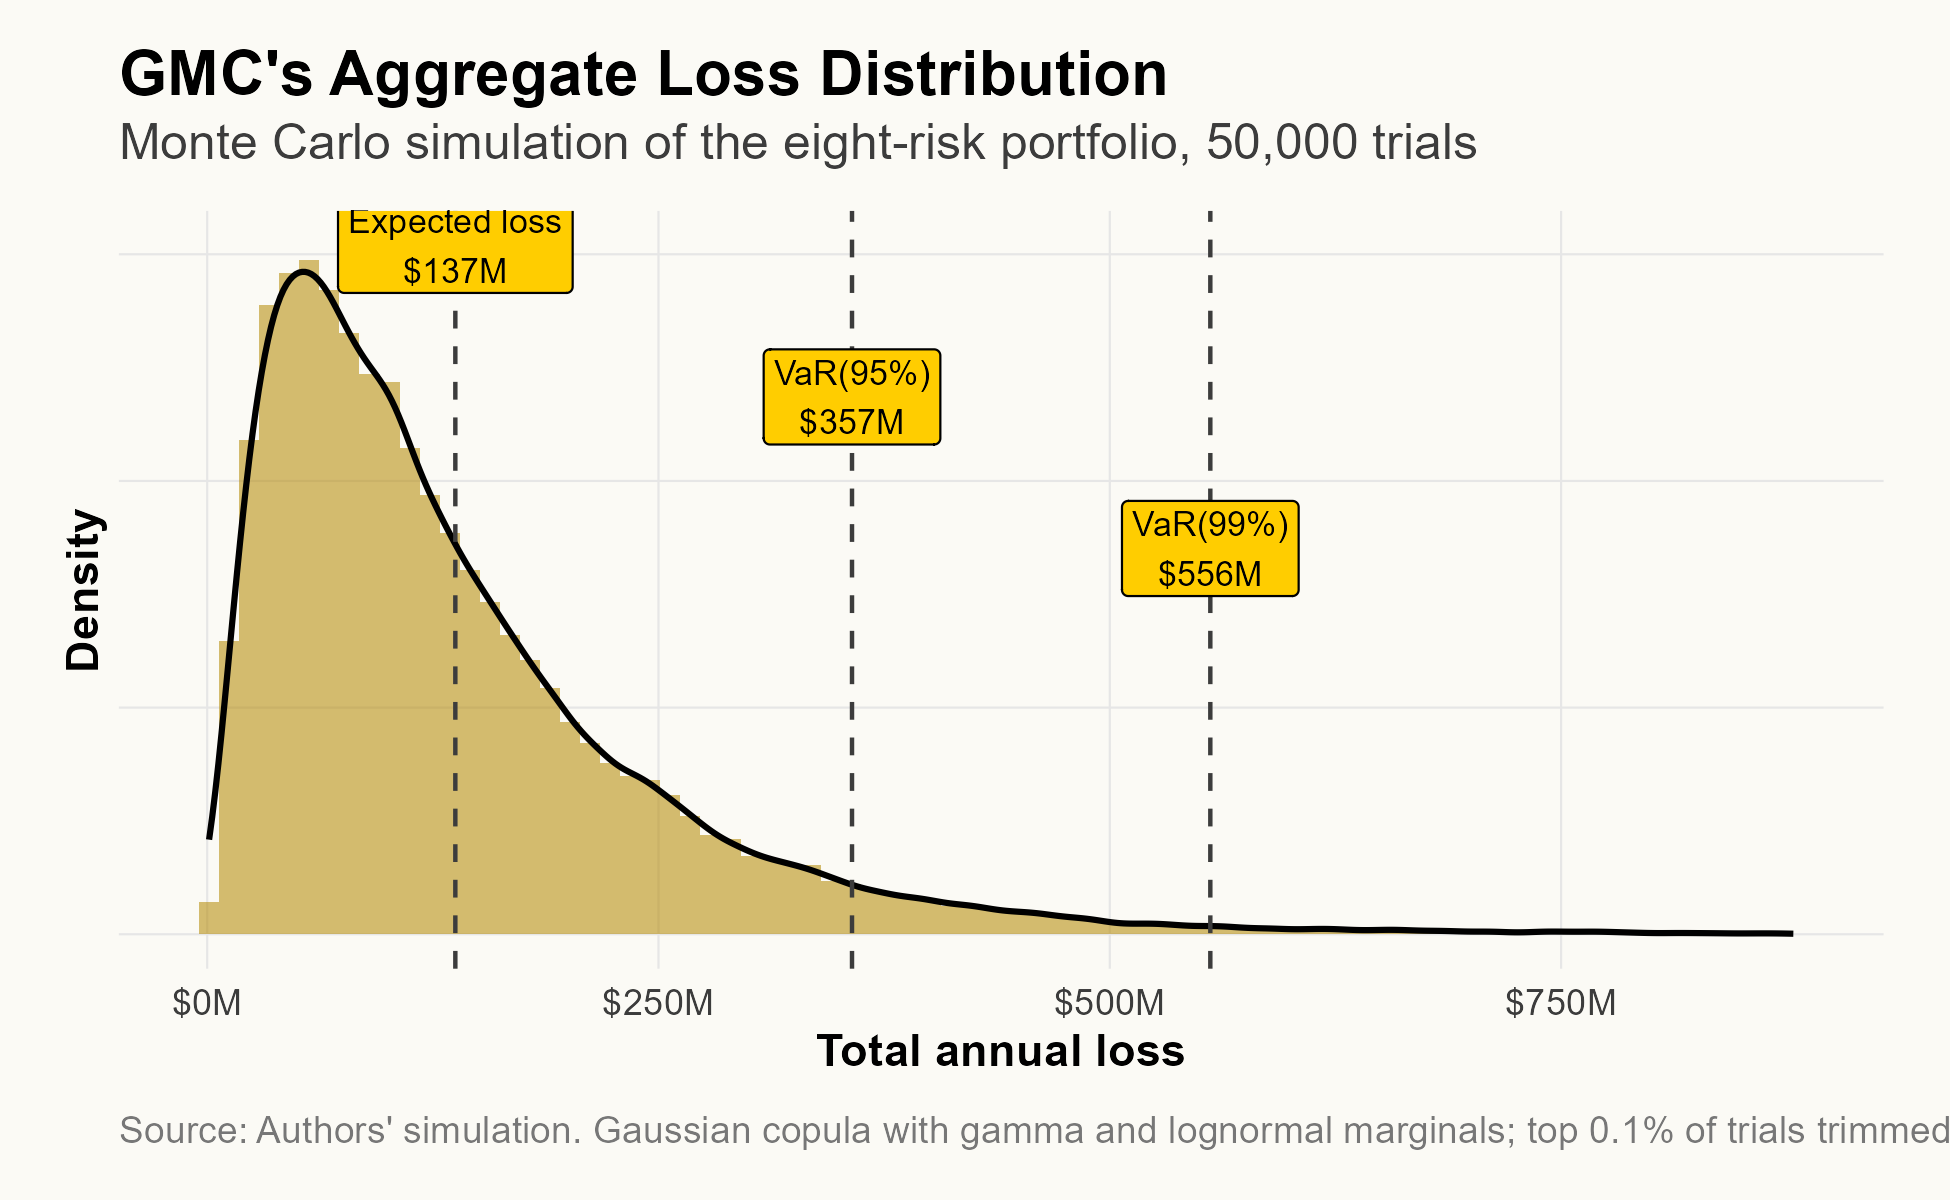
\includegraphics[width=\textwidth]{c6_aggregate_loss.png}
  \caption{GMC's simulated aggregate loss distribution. The distribution is
  strongly right-skewed: expected loss is \$137M, but VaR(95\%) is \$357M and
  VaR(99\%) is \$556M, well beyond what a normal approximation would predict.}
  \label{fig:gmc-aggregate}
  \figurenote{Monte Carlo simulation with 50{,}000 trials using a Gaussian
  copula on the correlation matrix in Table~\ref{tab:gmc-correlations}, with
  gamma marginals for most risks and lognormal marginals for supply chain and
  cyber risk. The top 0.1\% of trials is trimmed for display.}
\end{figure}

\subsection{Stress Testing}
\label{subsec:gmc-stress}

GMC designs three stress scenarios\index{stress testing}.

\textbf{Stress Scenario 1: Severe global recession.} Customer credit losses
triple (\$75M \(\rightarrow\) \$225M); commodity prices spike then collapse
(\$80M \(\rightarrow\) \$140M); strategic risk rises as customers cancel
contracts (\$70M \(\rightarrow\) \$120M); correlations among R1, R3, R8 rise
to 0.70. \textbf{Total portfolio loss: \$475M.}

\textbf{Stress Scenario 2: Major supply chain disruption.} Supply chain
disruption at the extreme---a geopolitical event (\$200M); property damage
from the same event (\$80M); product liability rises as substitute parts cause
defects (\$90M); cyber risk rises amid operational chaos (\$80M).
\textbf{Total portfolio loss: \$510M.}

\textbf{Stress Scenario 3: Combined moderate stress.} All risks at their 90th
percentiles---worse than expected, but no single catastrophe. \textbf{Total
portfolio loss: \$380M.}

\textbf{Conclusions:} under normal conditions (VaR(95\%) = \$352M), GMC is
within appetite. Under severe recession, losses (\$475M) exceed appetite and
consume nearly a quarter of equity. Under the supply chain crisis, losses
(\$510M) threaten covenant compliance. Even combined moderate stress (\$380M)
slightly exceeds appetite, though it is survivable.

\subsection{Management Actions and Portfolio Optimization}
\label{subsec:gmc-actions}

Portfolio analysis drives a concrete agenda.

\textbf{Risk mitigation:}
\begin{itemize}\tightlist
  \item Purchase additional property insurance with higher limits, capping R4
        at \$20M
  \item Expand the supplier diversification program, targeting a 20\%
        reduction in R6 VaR
  \item Increase commodity hedging (R3) to reduce volatility
\end{itemize}

\textbf{Capital and appetite:}
\begin{itemize}\tightlist
  \item Maintain current capital (\$2B equity) given the thin \$23M margin
        against the appetite limit
  \item Defer acquisition plans until portfolio risk falls---any new
        acquisition would push VaR above appetite
  \item Request board approval for a temporary appetite increase to \$425M if
        a strategic opportunity arises, with a 12-month plan to return
\end{itemize}

\textbf{Monitoring:}
\begin{itemize}\tightlist
  \item Quarterly portfolio VaR reporting to the board risk committee, with
        trend analysis
  \item Semi-annual stress testing with updated scenarios
  \item Ongoing monitoring of correlation changes
\end{itemize}

\textbf{Capital allocation and performance:}
\begin{itemize}\tightlist
  \item Allocate economic capital by marginal VaR contribution: Automotive
        45\% (\$540M), Industrial 35\% (\$420M), Consumer 20\% (\$240M)
  \item Measure RAROC per segment against a 12\% hurdle
  \item Include a risk-adjusted return metric in segment leaders' incentive
        compensation
\end{itemize}

\textbf{Result:} portfolio risk management transforms GMC's risk function from
a compliance exercise into a strategic tool informing capital allocation,
mitigation priorities, and growth decisions. The board sees its total risk
position relative to appetite---which is precisely what enterprise risk
management\index{enterprise risk management (ERM)} is for.

\begin{center}\rule{0.5\linewidth}{0.5pt}\end{center}

% -----------------------------------------------------------------------
\begin{keytakeaways}
\item
  A risk portfolio is the totality of material risks the firm faces,
  considered together with their interdependencies.
\item
  Total portfolio risk depends on individual risk magnitudes, correlations
  among risks, and the number of risks---it is not the sum of the parts.
\item
  Diversification reduces portfolio risk when correlations are less than
  perfect; benefits of 30--50\% relative to simple summation are typical.
\item
  Correlation (\(\rho\)) measures linear dependence between risks, ranging
  from \(-1\) to \(+1\); most business risk pairs fall between 0 and 0.6.
\item
  Risk aggregation methods include simple summation (conservative upper
  bound), variance-covariance (efficient, assumes normality), Monte Carlo
  simulation (flexible, handles skewed distributions), and copulas (capture
  tail dependence).
\item
  Correlations rise under stress; tail dependence means diversification is
  weakest exactly when it is needed most---as Maersk's NotPetya experience
  demonstrated, latent common dependencies can convert apparently independent
  exposures into one correlated loss.
\item
  Portfolio VaR, economic capital, and stress test results provide the
  enterprise-level metrics needed to assess compliance with board risk
  appetite.
\item
  Marginal contribution analysis identifies how much each risk or business
  unit adds to portfolio VaR, enabling rational capital allocation and
  risk-adjusted performance measurement (RAROC).
\item
  Stress testing complements probabilistic measures by evaluating extreme
  scenarios---historical, hypothetical, and reverse stress tests.
\item
  Implementation requires integrated data, correlation estimation discipline,
  model validation, and organizational commitment; the hardest problems are
  organizational, not mathematical.
\end{keytakeaways}

This chapter completes the core ERM technical toolkit: identify risks
(Chapter~3), quantify them individually (Chapter~4), establish appetite
(Chapter~5), and aggregate risks into portfolio views (Chapter~6). Subsequent
chapters explore risk response strategies and organizational implementation.

% -----------------------------------------------------------------------
\begin{keyterms}
  \item[\keyterm{Aggregate loss distribution}]
    The probability distribution of total losses across all risks in the
    portfolio, reflecting individual distributions and their correlations.
  \item[\keyterm{Copula}]
    A mathematical function separating the modeling of individual risk
    distributions from the modeling of dependencies, allowing flexible
    structures including tail dependence.
  \item[\keyterm{Correlation (\(\rho\))}]
    A statistical measure of the degree to which two variables move together,
    ranging from \(-1\) (perfect negative) to \(+1\) (perfect positive), with
    0 indicating independence.
  \item[\keyterm{Correlation matrix}]
    A table showing pairwise correlations between all risks in a portfolio,
    with diagonal elements equal to 1.
  \item[\keyterm{Covariance}]
    The expected value of the product of two variables' deviations from their
    means; Covariance(X,Y) = Correlation(X,Y) \(\times\) SD(X) \(\times\)
    SD(Y).
  \item[\keyterm{Diversification benefit}]
    The reduction in total portfolio risk relative to the simple sum of
    individual risks, arising from imperfect correlation.
  \item[\keyterm{Diversification ratio}]
    The ratio of portfolio risk to the sum of individual risks; values below 1
    indicate diversification benefit.
  \item[\keyterm{Economic capital}]
    The capital required to remain solvent at a specified confidence level
    given the firm's total risk portfolio.
  \item[\keyterm{Marginal VaR}]
    The incremental contribution of an individual risk to total portfolio
    VaR---portfolio VaR with the risk minus portfolio VaR without it.
  \item[\keyterm{Materiality threshold}]
    Criteria determining which risks are significant enough for the portfolio,
    based on financial magnitude, strategic importance, or regulatory
    requirements.
  \item[\keyterm{Monte Carlo simulation}]
    A computational technique generating thousands of random scenarios to
    construct empirical distributions of portfolio outcomes, accounting for
    risk distributions and correlations.
  \item[\keyterm{Portfolio VaR}]
    Value at Risk for the entire portfolio---the threshold loss exceeded with
    only a specified probability, accounting for diversification.
  \item[\keyterm{Reverse stress testing}]
    Working backwards from failure to identify what combination of events
    would cause it, then assessing plausibility.
  \item[\keyterm{Risk aggregation}]
    The process of combining individual risks to estimate total enterprise
    risk, accounting for correlations and dependencies.
  \item[\keyterm{Risk-Adjusted Return on Capital (RAROC)}]
    Net income divided by allocated economic capital, enabling return
    comparisons across units with different risk profiles.
  \item[\keyterm{Risk portfolio}]
    The totality of all material risks an organization faces, considered
    together as an integrated system including exposures and
    interdependencies.
  \item[\keyterm{Risk register}]
    A structured database documenting all material risks with identification,
    ownership, exposure metrics, correlations, and controls.
  \item[\keyterm{Stress testing}]
    Analysis evaluating portfolio performance under specific adverse scenarios
    that probabilistic measures may not capture.
  \item[\keyterm{Tail dependence}]
    The tendency for extreme losses across multiple risks to occur together
    more frequently than normal-period correlation predicts; correlations
    increase during crises.
  \item[\keyterm{Variance-covariance aggregation}]
    A method for calculating portfolio variance from individual risk variances
    and covariances (or correlations), based on portfolio theory.
\end{keyterms}

% -----------------------------------------------------------------------
\begin{discussionquestions}
\item \textbf{Conceptual:} Explain why examining risks individually rather
  than as a portfolio can lead to poor risk management decisions. Provide two
  specific examples of insights that portfolio analysis reveals that
  individual risk analysis misses.

\item \textbf{Conceptual:} Distinguish between correlation and tail
  dependence. Why does tail dependence matter for risk management even if
  normal-period correlations are low? How does the Maersk NotPetya case
  illustrate the distinction?

\item \textbf{Calculation:} Two risks each have expected loss of \$20M and
  standard deviation of \$10M. Calculate portfolio expected loss and standard
  deviation under three correlation assumptions: \(\rho = 1.0\),
  \(\rho = 0.5\), and \(\rho = 0\). Interpret the diversification benefit in
  each case.

\item \textbf{Application:} A company's current portfolio has VaR(95\%) =
  \$150M. The company is evaluating two potential acquisitions, each with
  standalone VaR(95\%) = \$50M. Acquisition~A correlates 0.8 with the current
  portfolio; Acquisition~B correlates 0.2. Without detailed calculations,
  explain qualitatively which acquisition adds more to portfolio risk and why.

\item \textbf{Integration:} Explain how portfolio VaR relates to risk appetite
  (Chapter~5). If a company's appetite is ``maximum annual loss shall not
  exceed \$200M with 95\% confidence,'' how does the company use portfolio
  analysis to assess compliance?

\item \textbf{Comparison:} Compare simple summation, variance-covariance
  aggregation, and Monte Carlo simulation as aggregation methods. What are the
  advantages and limitations of each? When is each most appropriate?

\item \textbf{Interpretation:} A company calculates portfolio VaR(95\%) =
  \$120M using the variance-covariance method and \$145M using Monte Carlo.
  What might explain the difference? Should management be concerned?

\item \textbf{Case analysis:} In the Global Manufacturing Co.\ case
  (Section~\ref{sec:gmc-case}), the diversification benefit was \$188M (35\%
  reduction). Identify three specific risk pairs with low correlation that
  contributed most to this benefit and explain why their correlation is low.

\item \textbf{Critical thinking:} A board member says ``If we have limited
  risk capacity, we should eliminate or reduce every risk as much as
  possible.'' Using portfolio concepts, explain why this reflects flawed
  reasoning. What should the board focus on instead?

\item \textbf{Strategy:} A manufacturing company operates only in the United
  States. Management proposes expansion into Europe and Asia. Using portfolio
  concepts, explain how this expansion might actually reduce total firm risk
  even though it adds new risks (foreign exchange, political, operational
  complexity). Under what conditions would expansion increase risk?

\item \textbf{Stress testing:} Design three stress test scenarios for a
  regional bank's risk portfolio. For each, identify which risks would be
  affected and how correlations might change under stress. Explain why these
  scenarios are more informative than relying solely on VaR.

\item \textbf{Organizational:} You are the newly appointed CRO of a company
  that has traditionally managed risks in functional silos (Treasury,
  Insurance, Operations). The CEO has asked you to implement portfolio risk
  management. Identify three major organizational or cultural challenges you
  expect and propose specific strategies to overcome each.
\end{discussionquestions}

% -----------------------------------------------------------------------
\begin{minicase}{Portfolio Risk Exercise --- TechRetail Corp}

\textbf{Scenario:} You are the risk analyst for \textbf{TechRetail Corp}, an
e-commerce and logistics company. The company has identified six material
risks (Table~\ref{tab:techretail-risks}) and estimated their correlations
(Table~\ref{tab:techretail-correlations}).

\begin{ermtable}{TechRetail's material risks}[tab:techretail-risks]
\begin{tabular}{@{}cllrr@{}}
\toprule
\textbf{ID} & \textbf{Risk Name} & \textbf{Expected Loss} &
\textbf{Std.\ Dev.} & \textbf{VaR(95\%)} \\
\midrule
R1 & Cyber/data breach        & \$15M & \$25M & \$60M \\
R2 & Warehouse accidents      & \$8M  & \$12M & \$28M \\
R3 & Delivery vehicle crashes & \$10M & \$15M & \$35M \\
R4 & Product liability        & \$12M & \$18M & \$42M \\
R5 & IT system failure        & \$5M  & \$10M & \$22M \\
R6 & Reputational damage      & \$7M  & \$20M & \$45M \\
\bottomrule
\end{tabular}
\end{ermtable}

\begin{ermtable}{TechRetail's correlation matrix}[tab:techretail-correlations]
\begin{tabular}{@{}lcccccc@{}}
\toprule
 & \textbf{R1} & \textbf{R2} & \textbf{R3} & \textbf{R4} & \textbf{R5} &
\textbf{R6} \\
\midrule
R1 & 1.00 & 0.15 & 0.10 & 0.20 & 0.70 & 0.60 \\
R2 & 0.15 & 1.00 & 0.40 & 0.30 & 0.10 & 0.20 \\
R3 & 0.10 & 0.40 & 1.00 & 0.50 & 0.10 & 0.25 \\
R4 & 0.20 & 0.30 & 0.50 & 1.00 & 0.15 & 0.70 \\
R5 & 0.70 & 0.10 & 0.10 & 0.15 & 1.00 & 0.50 \\
R6 & 0.60 & 0.20 & 0.25 & 0.70 & 0.50 & 1.00 \\
\bottomrule
\end{tabular}
\end{ermtable}

TechRetail's risk appetite: ``Portfolio VaR(95\%) shall not exceed \$180M.''

\medskip
\textbf{Part~1: Simple Aggregation (10 points).} Calculate total portfolio VaR
using simple summation (assuming perfect correlation). Does this exceed risk
appetite? By how much?

\medskip
\textbf{Part~2: Correlation Analysis (20 points).}
\begin{enumerate}[label=\alph*)]\tightlist
  \item Identify the two risks with the highest correlation. Explain
        intuitively why these risks might be highly correlated given
        TechRetail's business.
  \item Identify the two risks with the lowest correlation. Explain why these
        risks are largely independent.
  \item Based on the correlation matrix, which two risks offer the greatest
        diversification benefit when combined? Justify your answer.
\end{enumerate}

\medskip
\textbf{Part~3: Portfolio Calculation (30 points).} Using the
variance-covariance method:
\begin{enumerate}[label=\alph*)]\tightlist
  \item Calculate portfolio expected loss (simple sum of individual expected
        losses)
  \item Calculate portfolio variance using:
        \(\text{Portfolio Variance} = \sum \sigma_i^2 +
        \sum\sum \rho_{ij}\,\sigma_i\,\sigma_j\) for all \(i \neq j\)
  \item Calculate portfolio standard deviation =
        \(\sqrt{\text{Portfolio Variance}}\)
  \item Estimate portfolio VaR(95\%) using the normal approximation:
        VaR = Expected Loss + 1.645 \(\times\) Portfolio SD
\end{enumerate}
(Note: For the full calculation, use a spreadsheet or calculator. Show at
least the setup and a few sample calculations even if you don't compute the
final number by hand.)

\medskip
\textbf{Part~4: Diversification Benefit (20 points).}
\begin{enumerate}[label=\alph*)]\tightlist
  \item Calculate the diversification benefit: Simple Sum VaR \(-\) Portfolio
        VaR (from Parts~1 and~3)
  \item Calculate diversification benefit as a percentage:
        \([1 - (\text{Portfolio VaR} / \text{Simple Sum VaR})] \times 100\%\)
  \item Is the portfolio VaR within risk appetite? How much risk capacity
        remains?
\end{enumerate}

\medskip
\textbf{Part~5: Strategic Decision (20 points).} TechRetail is considering
launching same-day drone delivery. The new service would add:

R7: Drone accidents --- Expected Loss \$6M, Standard Deviation \$15M,
VaR(95\%) estimated \$35M

Estimated correlations with existing risks:
\begin{itemize}\tightlist
  \item R1 (Cyber): 0.40 (drones depend on IT systems, vulnerable to cyber)
  \item R2 (Warehouse): 0.25 (some connection through logistics operations)
  \item R3 (Vehicle crashes): 0.60 (both transportation risks)
  \item R4 (Product liability): 0.45 (drone accidents could damage products)
  \item R5 (IT failure): 0.55 (drones heavily IT-dependent)
  \item R6 (Reputational): 0.50 (drone accidents attract media attention)
\end{itemize}

Without performing full calculations, answer qualitatively:
\begin{enumerate}[label=\alph*)]\tightlist
  \item How do you expect R7 to affect portfolio VaR? Will it increase by the
        full \$35M standalone VaR, or by less due to diversification? Explain
        your reasoning with reference to the correlations.
  \item Should TechRetail approve the new service from a risk portfolio
        perspective if it offers attractive returns? What additional analysis
        would you recommend before a final decision?
\end{enumerate}

\medskip
\textbf{Submission format:} You may use Excel, a calculator, or show work by
hand. Submit calculations, answers, and written explanations (2--3 pages
total). Partial credit for methodology even if calculations contain errors.

\end{minicase}

% -----------------------------------------------------------------------
\section*{Advanced Challenge: Monte Carlo Portfolio Simulation}
\addcontentsline{toc}{section}{Advanced Challenge: Monte Carlo Portfolio Simulation}

For students comfortable with Excel or programming (R/Python):

\textbf{Task:} Build a Monte Carlo simulation for TechRetail's 6-risk
portfolio:

\begin{enumerate}\tightlist
  \item In Excel, create correlated normal random variables for the 6 risks
        using the Cholesky decomposition method or Excel's built-in
        correlation tools
  \item For each simulation trial (at least 1{,}000 trials), generate
        correlated losses for all 6 risks and sum to get total portfolio loss
  \item From the simulated portfolio losses: calculate the mean (portfolio
        expected loss), the standard deviation (portfolio SD), and the 95th
        percentile (portfolio VaR(95\%)); create a histogram of the portfolio
        loss distribution
  \item Compare your Monte Carlo results to the variance-covariance results
        from the main exercise
  \item Write a brief summary (1 page) discussing: How closely do Monte Carlo
        and variance-covariance results agree? What are the advantages of
        Monte Carlo for this problem? How would you modify the simulation to
        better capture tail risk?
\end{enumerate}

\textbf{Optional extension:} Introduce non-normal distributions (e.g.,
lognormal for R1 cyber risk to capture right-skew) and observe how the
portfolio distribution changes.

% -----------------------------------------------------------------------
\section*{References}
\addcontentsline{toc}{section}{References}
\begingroup
\sloppy

\begin{hangparas}{1.5em}{1}

Columbia University School of International and Public Affairs. (2022).
\emph{NotPetya: A Columbia University case study.} Columbia SIPA.
\url{https://www.sipa.columbia.edu/sites/default/files/2022-11/NotPetya%20Final.pdf}

Committee of Sponsoring Organizations of the Treadway Commission. (2017).
\emph{Enterprise risk management---Integrating with strategy and performance.}
COSO. \url{https://www.coso.org/}

Greenberg, A. (2018a, August 22). The untold story of NotPetya, the most
devastating cyberattack in history. \emph{WIRED}.
\url{https://www.wired.com/story/notpetya-cyberattack-ukraine-russia-code-crashed-the-world/}

Greenberg, A. (2018b, February 15). The White House blames Russia for
NotPetya, the ``most costly cyberattack in history.'' \emph{WIRED}.
\url{https://www.wired.com/story/white-house-russia-notpetya-attribution/}

International Organization for Standardization. (2018). \emph{ISO~31000:2018
Risk management---Guidelines} (2nd~ed.). ISO.
\url{https://www.iso.org/standard/65694.html}

Los Angeles Times. (2017, August 17). Maersk cyberattack closes Port of Los
Angeles terminal. \emph{Los Angeles Times}.
\url{https://www.latimes.com/business/la-fi-maersk-cyberattack-20170817-story.html}

Markowitz, H. (1952). Portfolio selection. \emph{The Journal of Finance,
7}(1), 77--91.

\end{hangparas}

\endgroup
\end{document}
